\chapter{Versuch 1 - Bestimmung der Tonhöhe eines akustischen Signals}
\label{chap:VERSUCH_1}


\section{Fragestellung, Messprinzip, Aufbau, Messmittel}
\label{chap:VERSUCH_1_FRAGESTELLUNG}

\subsection*{Fragestellung}
	In diesem Versuch geht es darum einen einzelnen Ton eines Musikinstruments mit einem Mikrofon aufzunehmen.
Das daraus resultierende Signal soll dann in sein Spektrum zerlegt und dargestellt werden.
Dadurch soll ein praktisches Verständnis für die Messung von Tonsignalen und der Fourieranalyse vermittelt werden.
	
\subsection*{Messprinzip}
Die Fourieranalyse ist ein essenzielle Methoden für die Signalverarbeitung. Sie erlaubt es die Grundfrequenz sowie die Obertöne einer Schwingung zu ermitteln.

\subsection*{Aufbau}

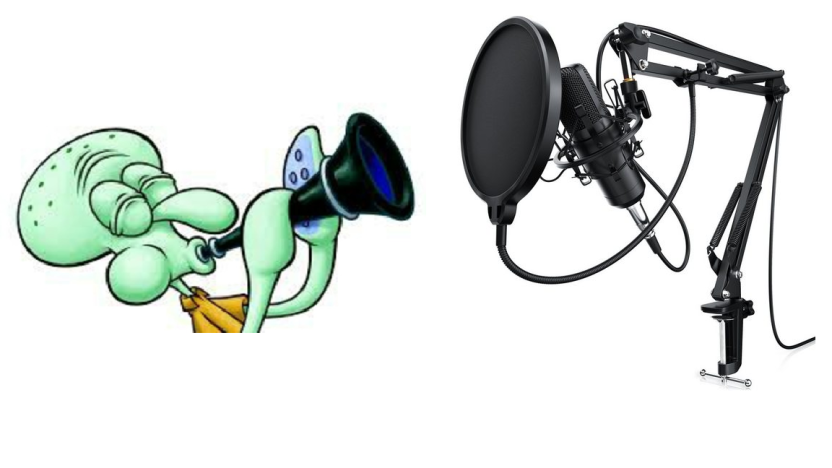
\includegraphics[scale=0.4]{media/Versuchaufbau.png}
\label{Abb:Aufbau}


\subsection*{Messmittel}
\begin{itemize}
	\item Mikrophon
	\item Klanguelle (Klarinette)
\end{itemize}

\section{Messwerte}
\label{chap:VERSUCH_1_MESSWERTE}

Zwei Schwinungen, aus den späteren abschnitten (die ersten 50.000 Werte wurden übersprungen, weil das Signal zu verworren war)
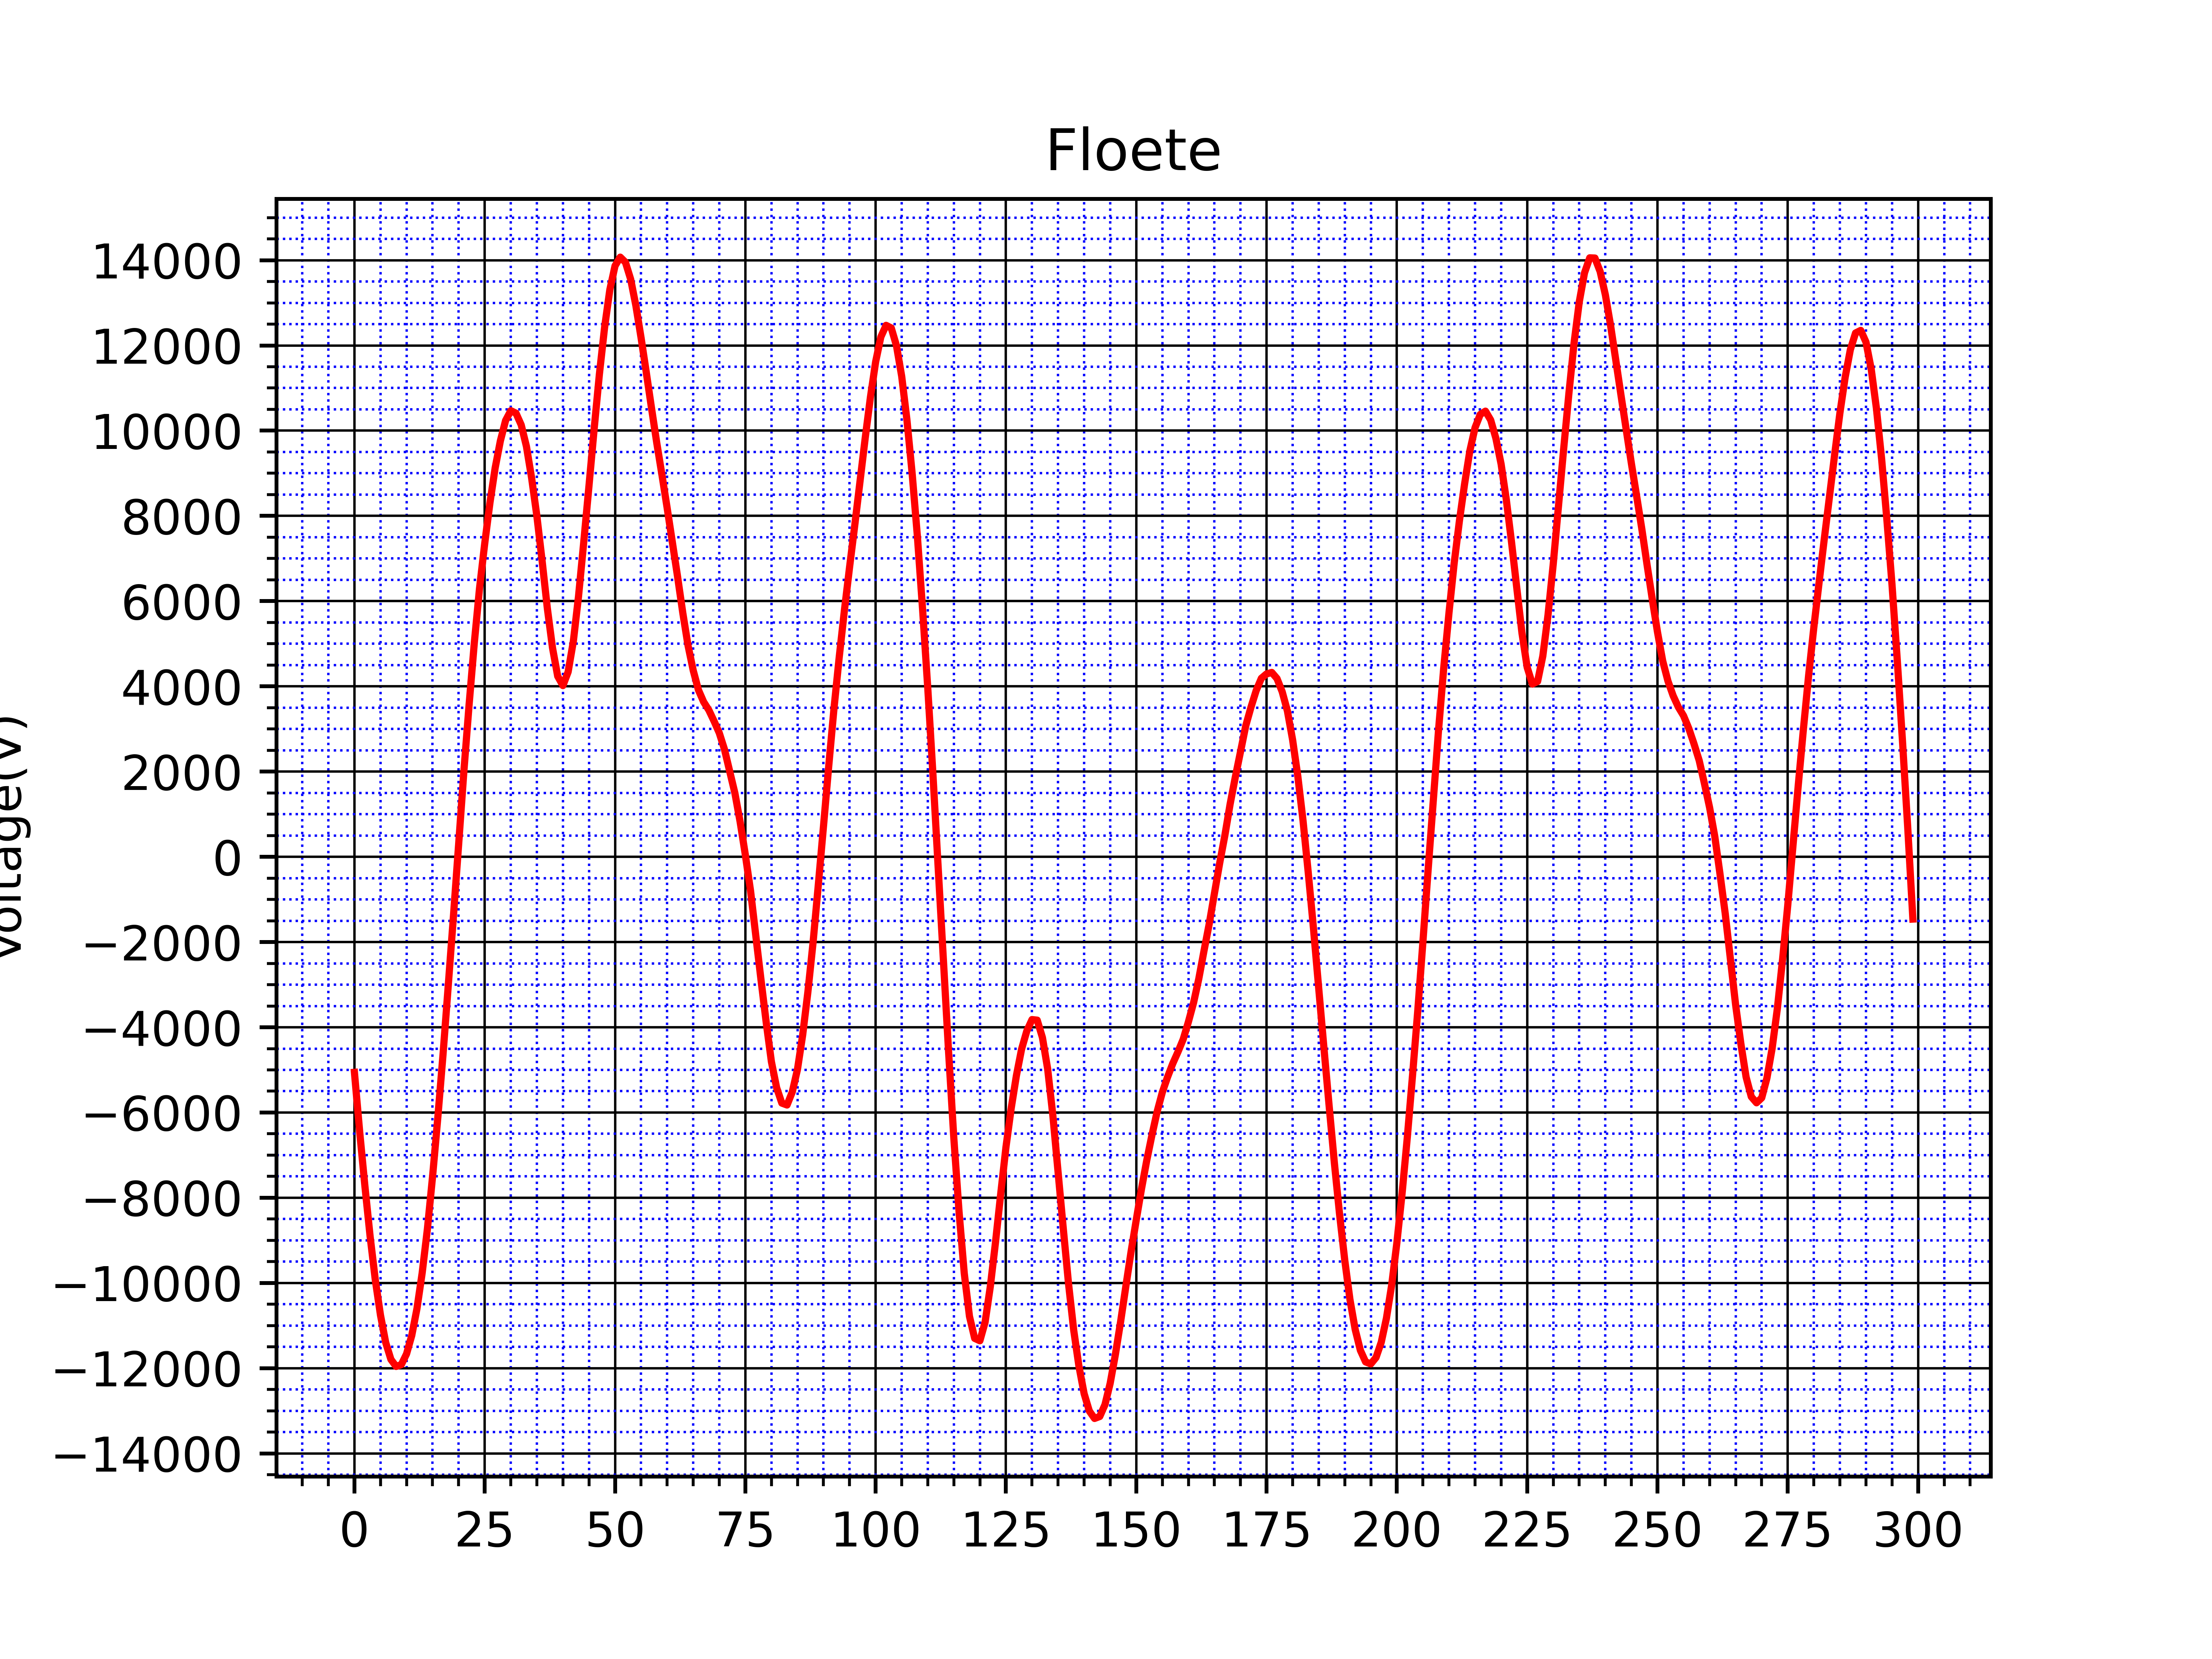
\includegraphics[scale=0.05]{media/Signal_Raster.png}

Die Werte auf der X-Achste stehen hierbei für Abtastpunke über die Zeit und sind daher einheitslos.

\section{Auswertung}
\label{chap:VERSUCH_1_AUSWERTUNG}

\subsection*{Randdaten}

Vor Beginn der eigentlichen Auswertung werden erst  mal die Randdaten festgelegt. Das Signal wurde mittels des Beispielprogramms audioSample.py aufgenommen und abgespeichert. Dabei hat das Programm über einen Gesamtzeitraum von 225280 Frames gemessen und in dieser wurden 44100 Frames die Sekunde gemessen.
Das bedeutet die \textbf{Signallänge} beträgt 225280 und die \textbf{Abtastfrequenz} beträgt 44100 Hz.
Daraus lässt sich auch die Messdauer berechnen:
\begin{equation}
	L = \frac{M}{a} = \frac{225280}{44100 Hz} = 5,1084 s
\end{equation}
\begin{itemize}
	\item L = Signaldauer = 5,1084 s
	\item M = Signallänge = 225280
	\item a = Abtastfrequenz = 441000 Hz 
\end{itemize}

Das \textbf{Abtastintervall} ergibt sich aus:

\begin{equation}
	\Delta t = \frac{1}{a} = 0,000022676 s
\end{equation}
\begin{itemize}
	\item $\Delta t$ = Abtastintervall
\end{itemize}

Das Abtastintervall ist also 0,000022676 s oder 0,022676 ms.

\subsection*{Grundperiode und Grundfrequenz}

Um die Grundfrequenz ermitteln zu können muss zu nächst die Grundperiode bekannt sein.
Grundperiode: Zeitliche dauer bis sich die Schwingung wiederholt. Sie muss folglich aus den Plot abgelesen werden:
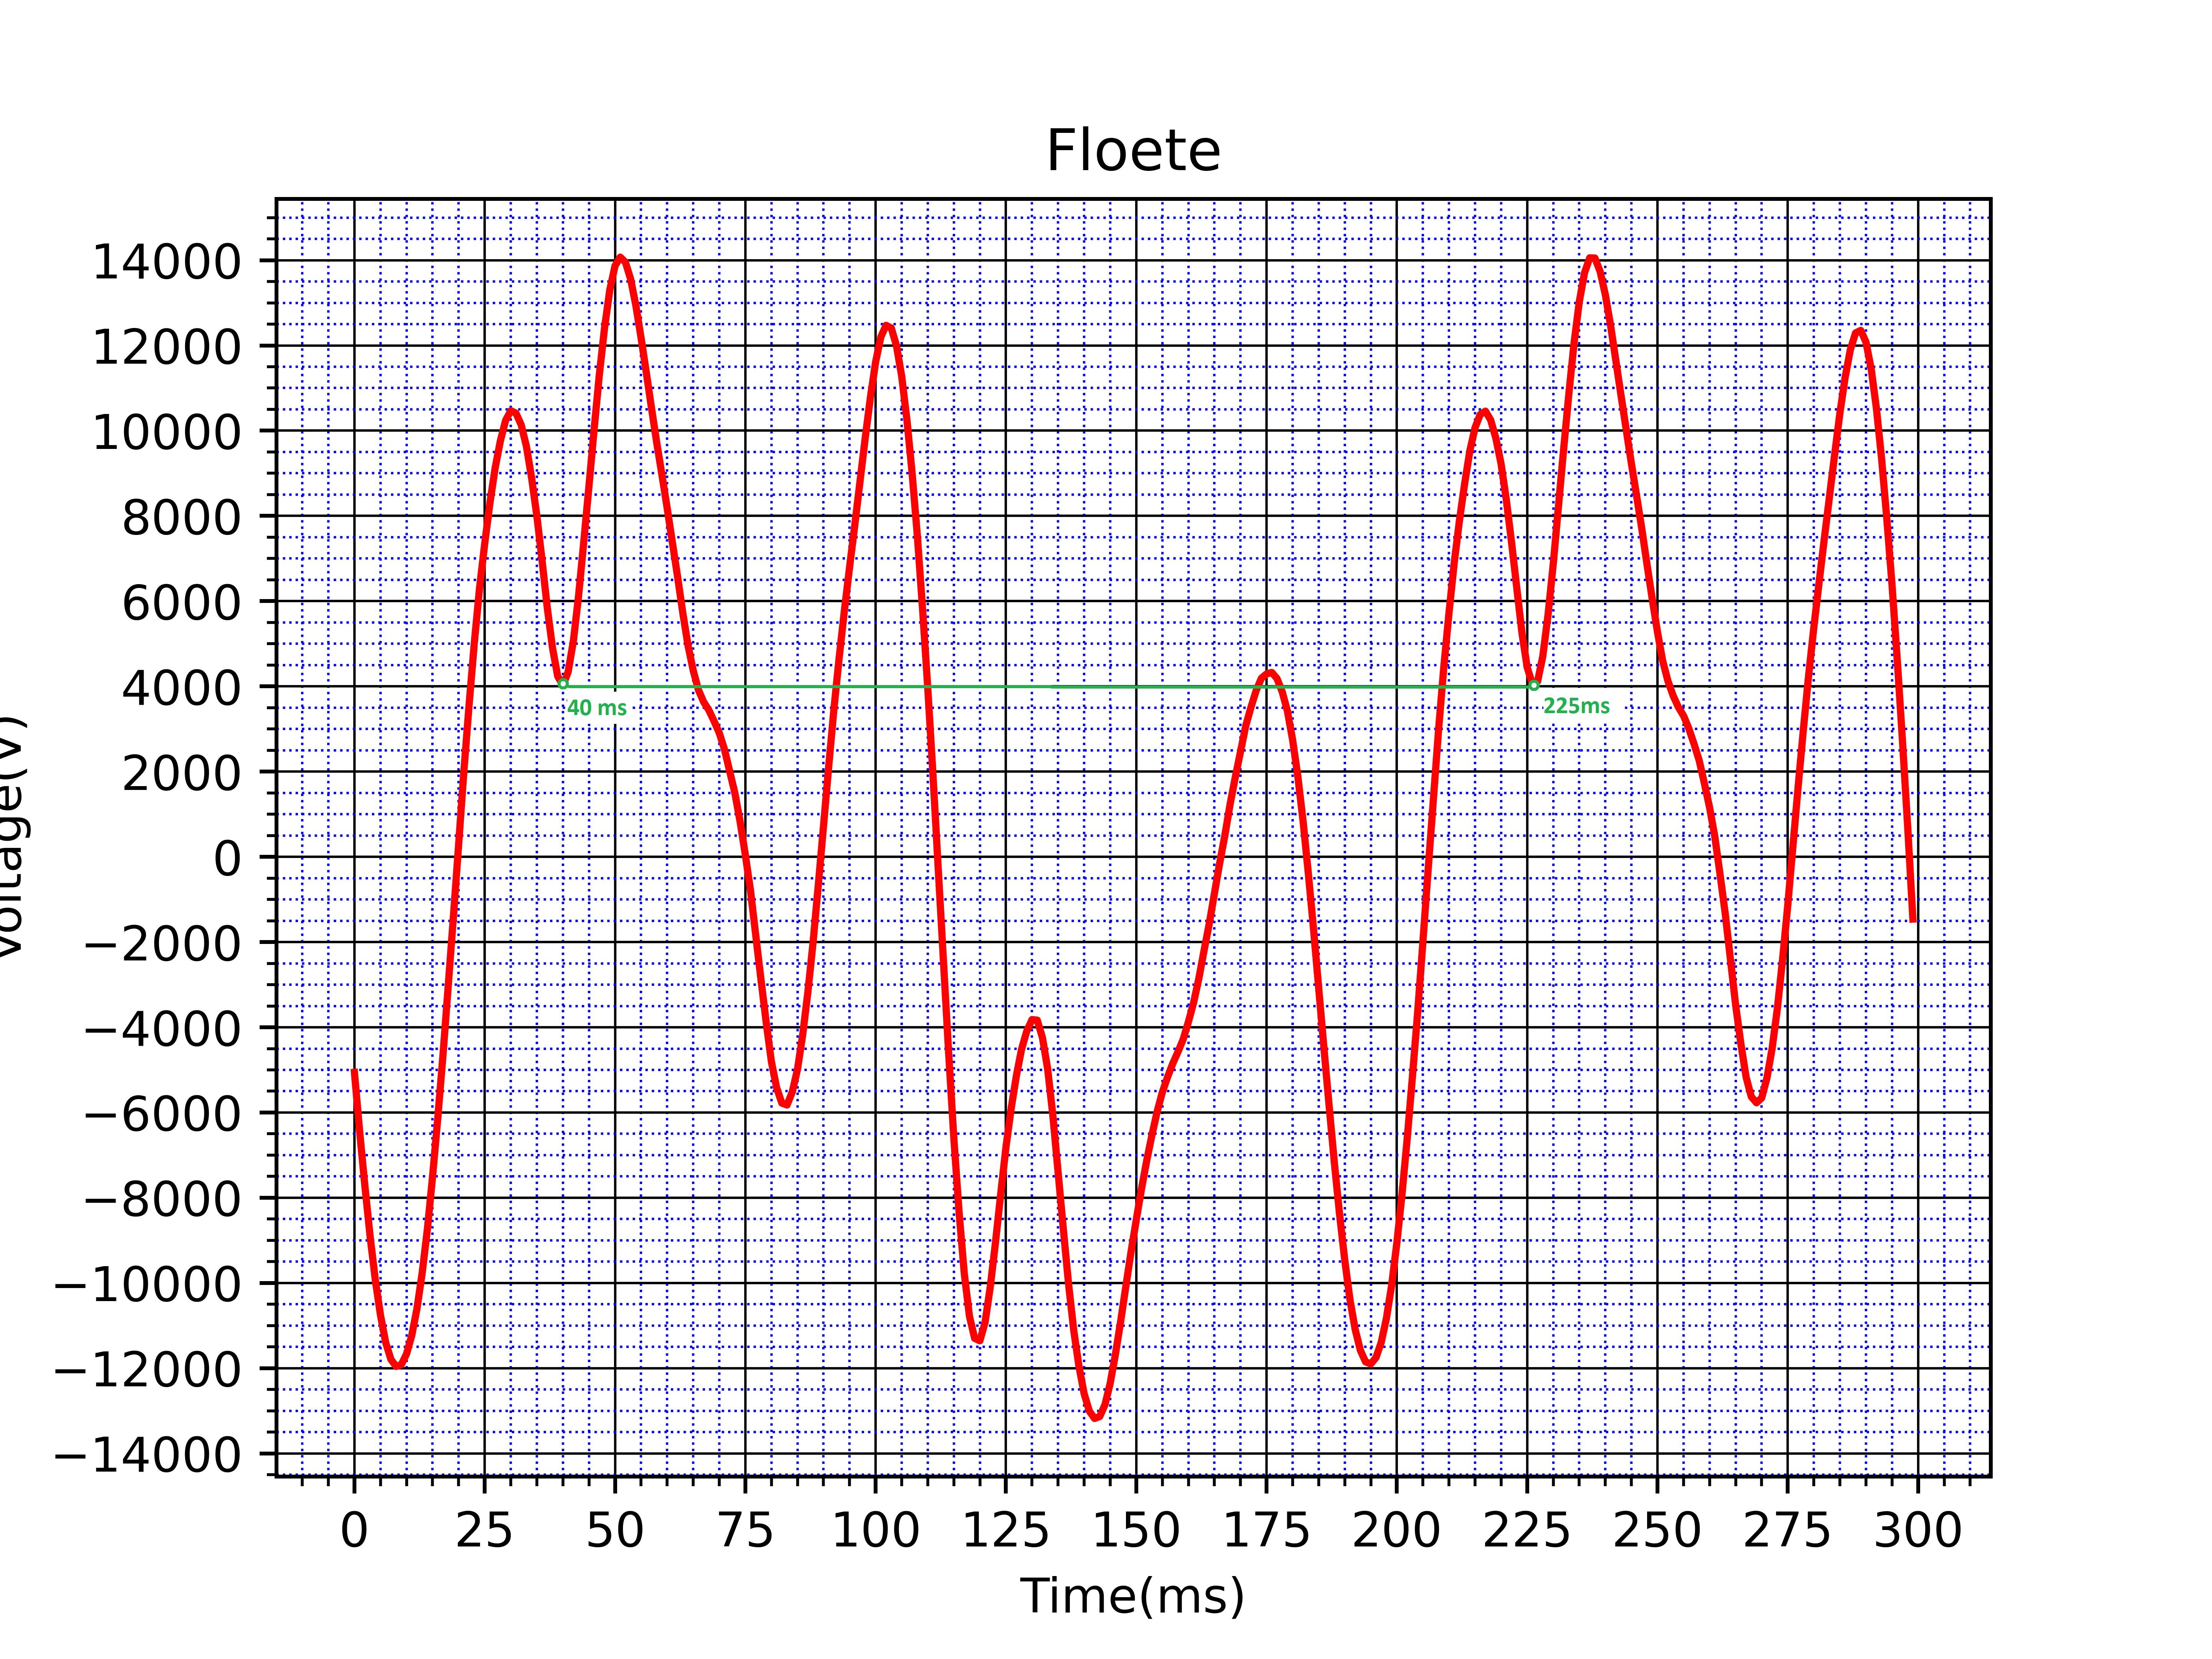
\includegraphics[scale=0.05]{media/Signal_Raster_Periode.png}

An der Graphik lässt sich erkennen das $ Grundperiode = 225 - 40 = 185 $ ist.
Da es sich bei 185 um die Anzahl von Abtastpunkten handelt ist es noch nötig sie in sekunden umzurechnen:

\begin{equation}
	G = Abtastpunkte \ast \Delta t = 185 \ast 0,000022676 s
\end{equation}
\begin{itemize}
	\item G = Grundperiode = 0,004195 s 
\end{itemize}

Nun lässt sich auch die Frequenz berechnen. 
Sie ergibt sich aus:
\begin{equation}
	f =  \frac{c}{t} = \frac{1}{0,004195 s} = 238,38 Hz
\end{equation}
\begin{itemize}
	\item f = Grundfrequenz in Hz 
	\item n = Anzahl Schwingungen
	\item t = Gemessener Zeitraum in s
\end{itemize}

Die Grundfrequenz beträgt also 238,38 Hz.

\subsection*{Fouriertransformation}

Um nun zu dem gemessenen Signal das Spektrum zu ermitteln wird die Funktion fft von numpy angewandt.
daraus ergibt sich folgendes Spektrum:

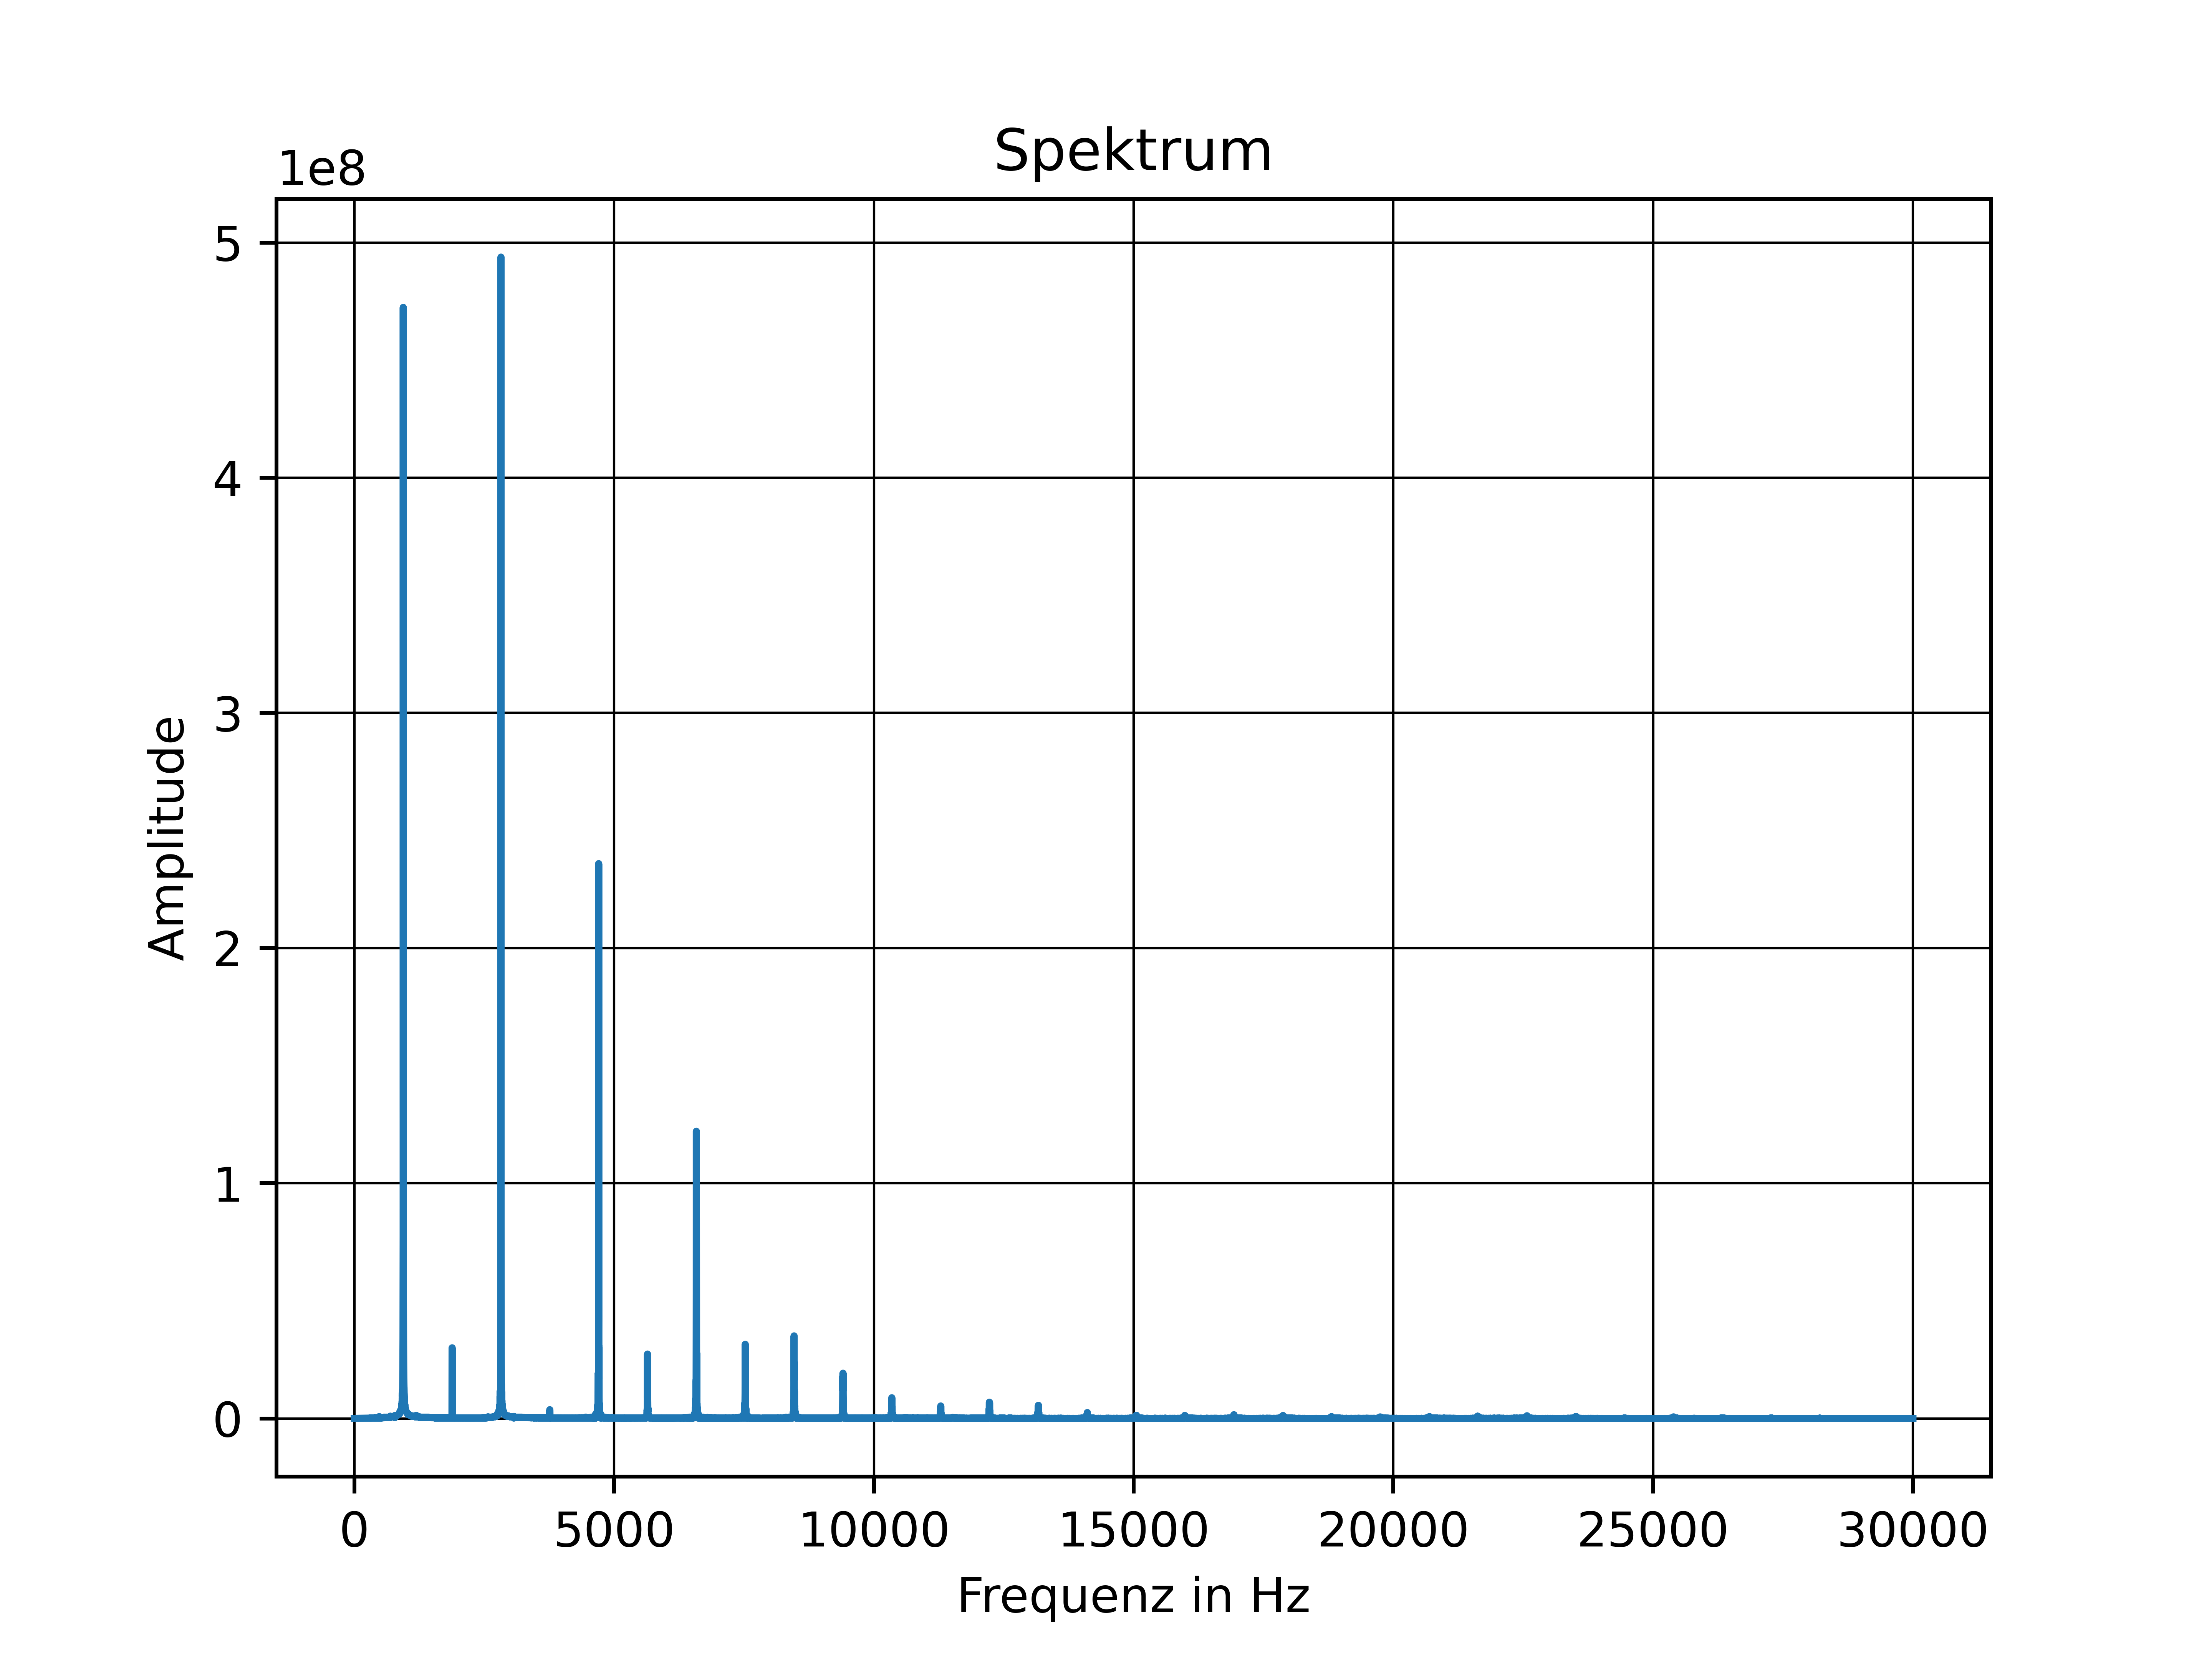
\includegraphics[scale=0.5]{media/Fouriertranformierte.png}

\section{Interpretation}
\label{chap:VERSUCH_1_INTERPRETATION}


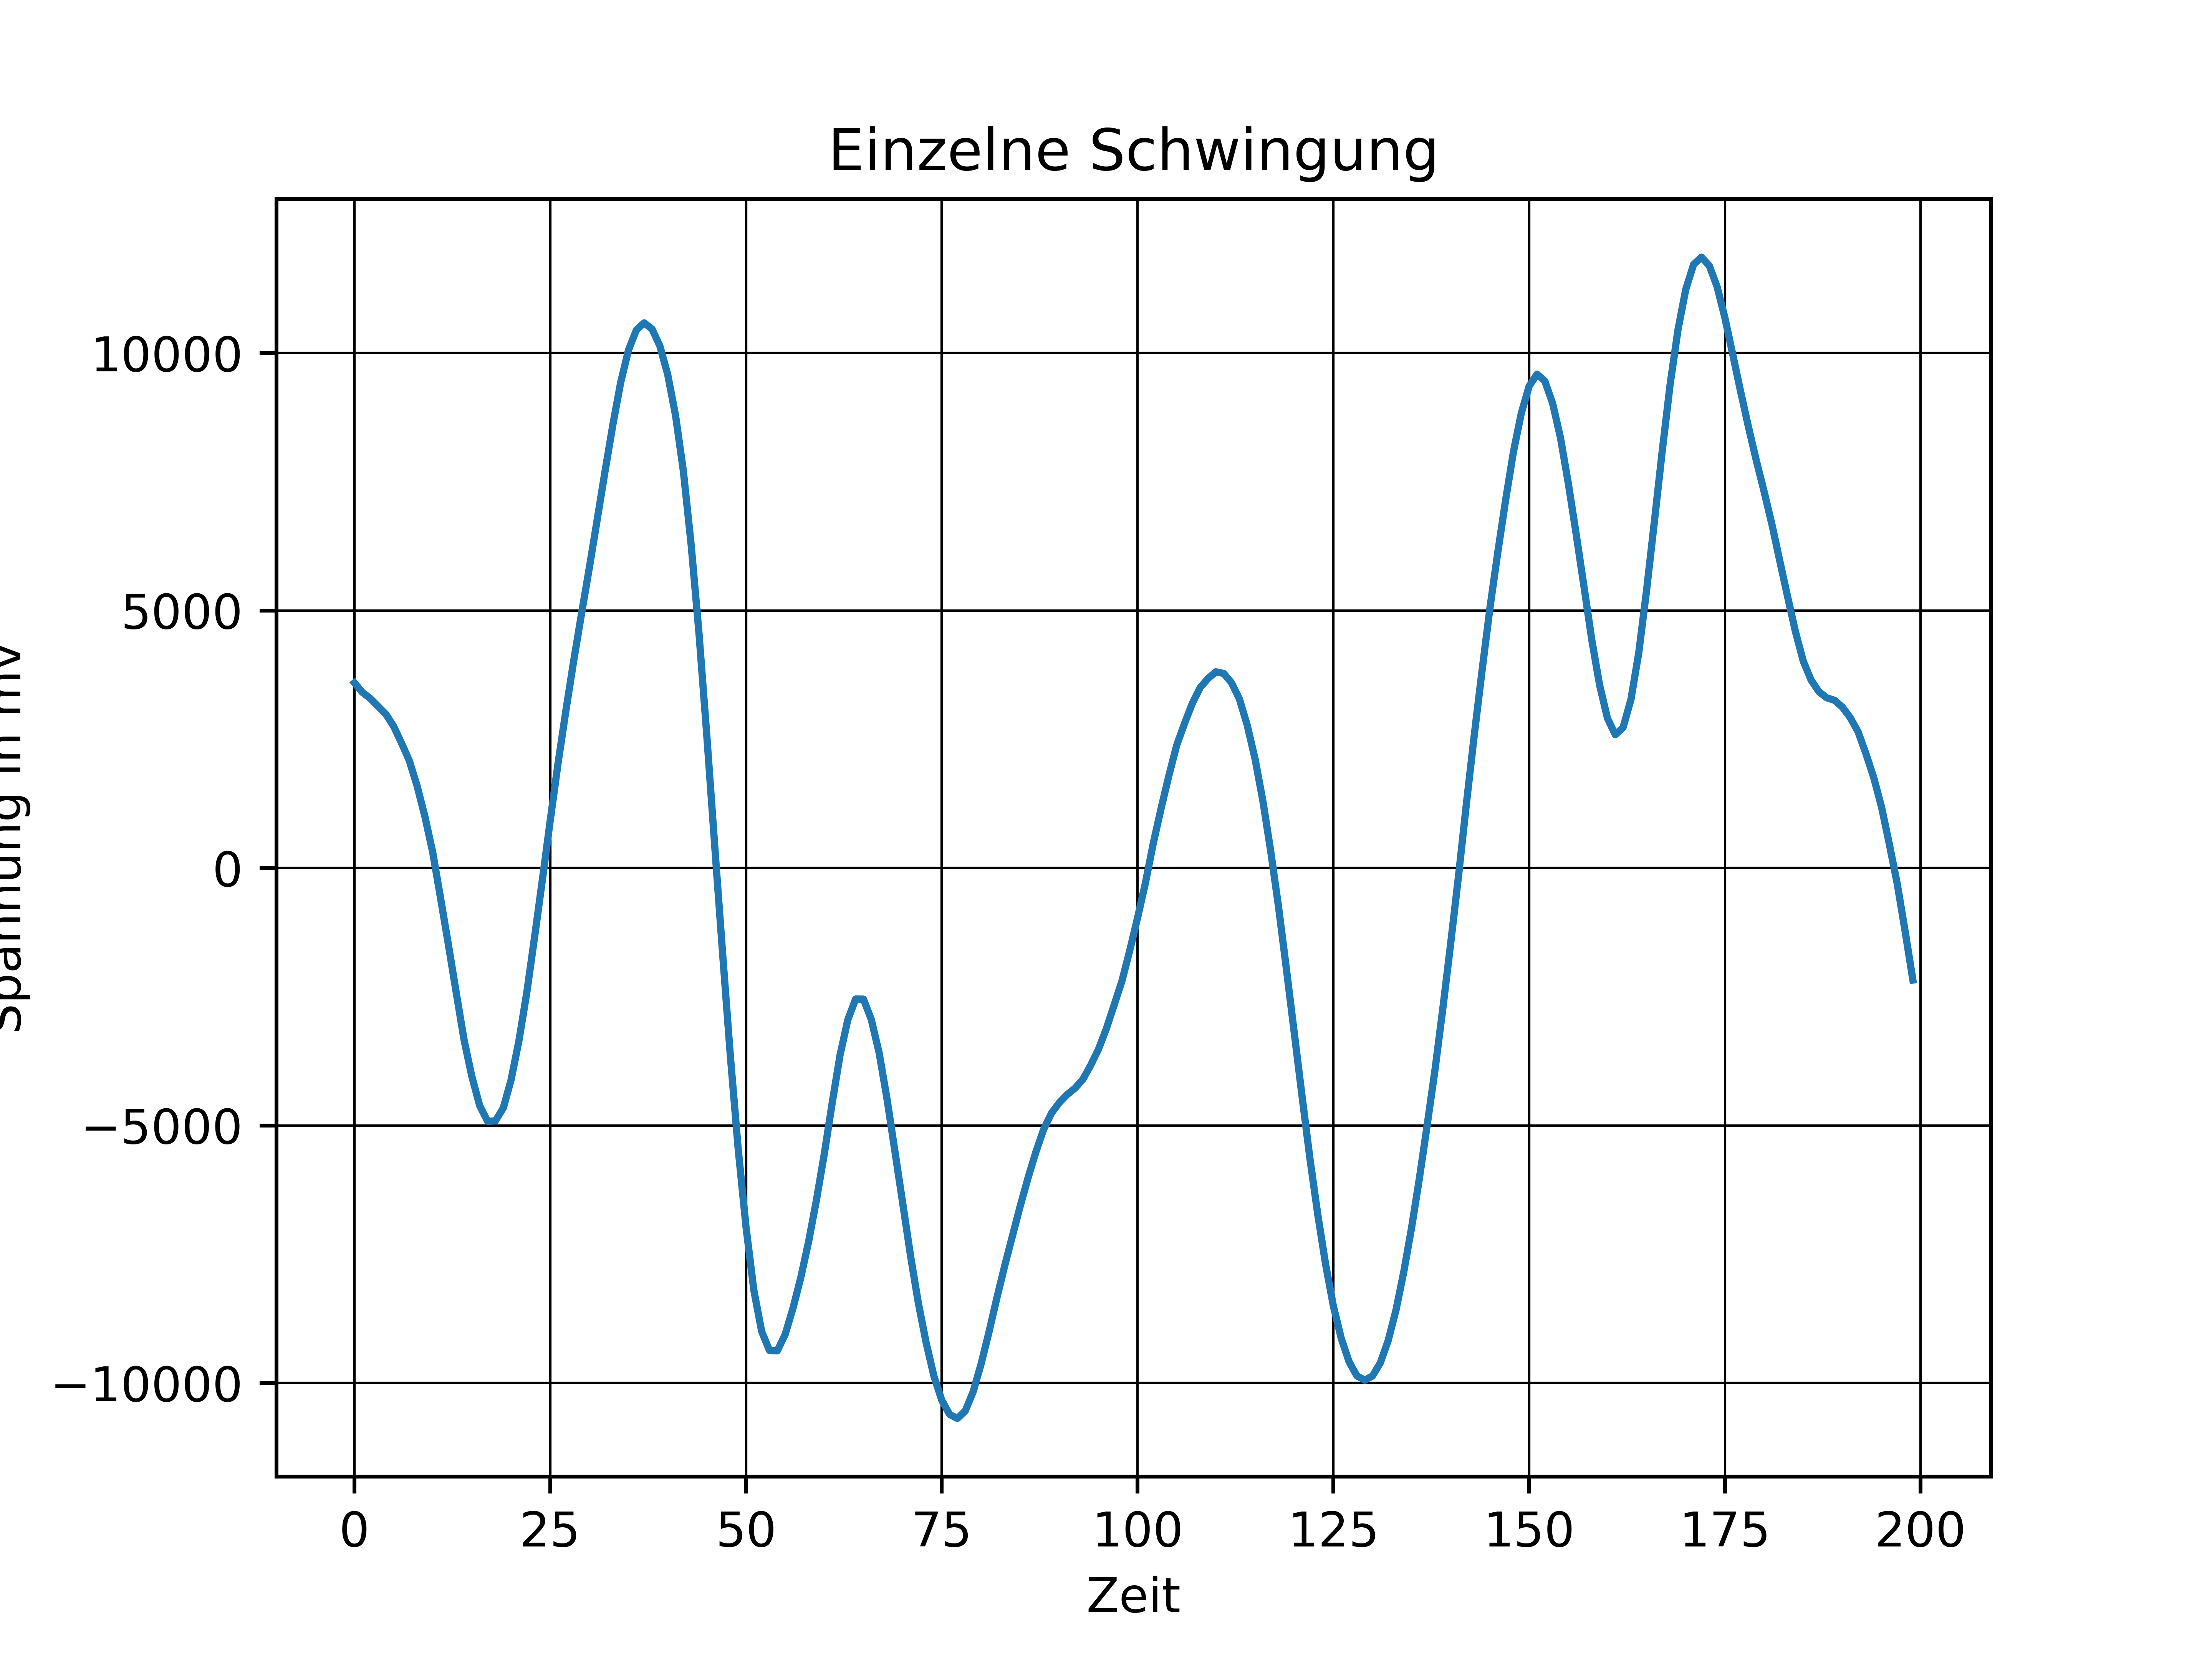
\includegraphics[scale=0.5]{media/singleperiod.png}
\label{fig: Einzelne Schwingung}
\captionof{figure}{fig:Single}

In der Abbildung \ ist sehr gut zu sehen dass sich die von uns zuvor berechnete Grundfrequenz
bei ca. 238Hz befindet. Da es sich um ein periodisches Signal handelt sind die folgenden Harmonischen Schwingungen bei vielfachen von 238Hz zu sehen, welche jedoch auf Grund von Messungenauigkeiten und Rundungsfehlern etwas davon abweichen.